\clearpage
\section{Constraints on proton structure}
\label{sec:protonPDFs}

By means of the strategy outlined in Sect.~\ref{sec:settings}, here we study the constraints that differential neutrino DIS
cross-section measurements at the LHC have on the quark and gluon substructure of the proton.
%
In this section we assume an isoscalar free-nucleon target and neglect non-isoscalarity effects and nuclear modifications,
which are instead considered in Sect.~\ref{sec:nuclearPDFs}.
%
We present results first for the Hessian profiling of the PDF4LHC21 combination of global PDF sets
and second for the inclusion in the Monte Carlo fit NNPDF4.0.
%
We study the dependence on the result with respect to the choice of fitted dataset, the experiment considered,
the modelling of experimental systematic uncertainties, and the availability or not of charged lepton separation.

\subsection{Impact on PDF4LHC21}
\label{sec:pdf4lhc21}

For the Hessian profiling studies following the procedure of Sect.~\ref{sec:profiling}, the prior PDF set is taken to
be PDF4LHC21 NNLO, a Monte Carlo combination~\cite{Watt:2012tq,Carrazza:2015hva} of three global PDF sets (CT18~\cite{Hou:2019efy},
MSHT20~\cite{Bailey:2020ooq}, and NNPDF3.1~\cite{NNPDF:2017mvq}) for which Hessian
representations~\cite{Gao:2013bia,Carrazza:2015aoa} are also provided.
%
PDF4LHC21, being based on the combination of three modern global fits, provides a reasonable representation
of our current understanding of the proton PDFs.
%
We profile PDF4LHC21 with the various sets of LHC neutrino pseudo-data and assess the reduction
of PDF uncertainties in each case.
%
In this analysis, a tolerance of $T = \sqrt{\Delta \chi^2}=3$ is adopted, which is the average tolerance
used in the CT18 and MSHT20 Hessian determinations.
%
Note that we use a consistent perturbative accuracy in the prior PDF set and in the theoretical calculations.

In the following, we first compare the impact on PDF4LHC21 of a baseline LHC neutrino dataset and subsequently
we assess the stability of this result with respect to a range of variations of its input.

\paragraph{Baseline results.}
%
The baseline dataset is defined as follows.
%
We consider the FASER$\nu$2 experiment integrated over the full duration of the HL-LHC data-taking period,
we account both for inclusive and charm production structure functions, we consider the scenario
in which systematic errors can be neglected, and we allow for charge separation of the outgoing lepton.
%
This baseline result therefore represents the best-case scenario and quantifies the maximum impact that can be expected
on the PDFs: we then assess to which extent variations of these input choices degrade the reach of the pseudo-data.

Fig.~\ref{fig:profiling_baseline} displays the fractional uncertainties at the 68\% confidence level
for the up and down valence quarks, total quark singlet, strangeness, charm, and gluon PDFs
in PDF4LHC21 compared to the results of its profiling with this baseline LHC neutrino dataset, namely
FASER$\nu$2 with only statistical errors, both inclusive and charm structure functions,  and charge flavour
separation.
%
The same style of PDF comparisons will be adopted through this section.
%
Results are shown at $Q^2 = 10^4 \, \textrm{GeV}^2$ and the residual shift in central values
arising from the profiling is ignored.

%%%%%%%%%%%%%%%%%%%%%%%%%%%%%%%%%%%%%%%%%%%%%%%%%%%%%%%%%%%%%%%%%%%%%5
\begin{figure}[t]
\centering
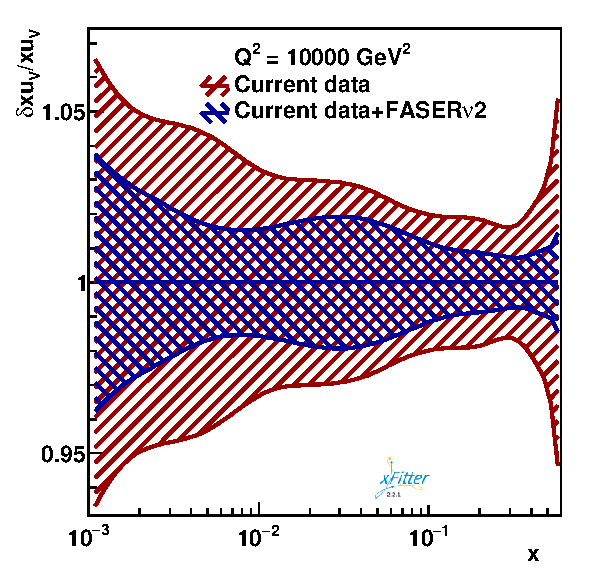
\includegraphics[width=0.32\textwidth]{plots/proton_fasernu2/inclusive+charm_chargediscrimination/statOnly_FASERv2_q2_10000_pdf_uv_ratio.pdf}
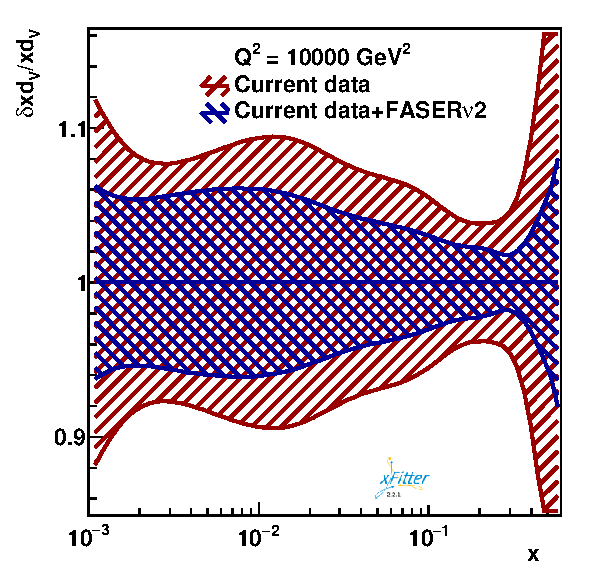
\includegraphics[width=0.32\textwidth]{plots/proton_fasernu2/inclusive+charm_chargediscrimination/statOnly_FASERv2_q2_10000_pdf_dv_ratio.pdf}
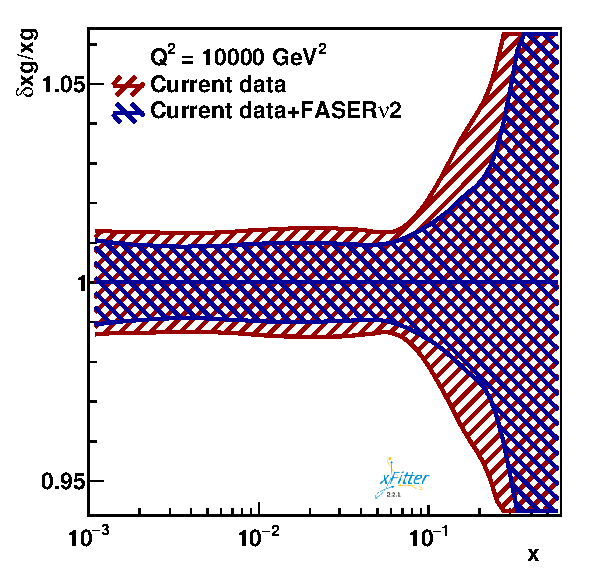
\includegraphics[width=0.32\textwidth]{plots/proton_fasernu2/inclusive+charm_chargediscrimination/statOnly_FASERv2_q2_10000_pdf_g_ratio.pdf}\\
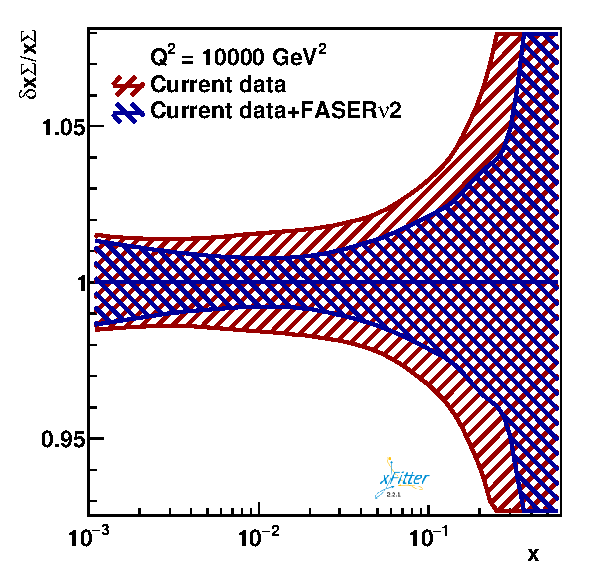
\includegraphics[width=0.32\textwidth]{plots/proton_fasernu2/inclusive+charm_chargediscrimination/statOnly_FASERv2_q2_10000_pdf_Sea_ratio.pdf}
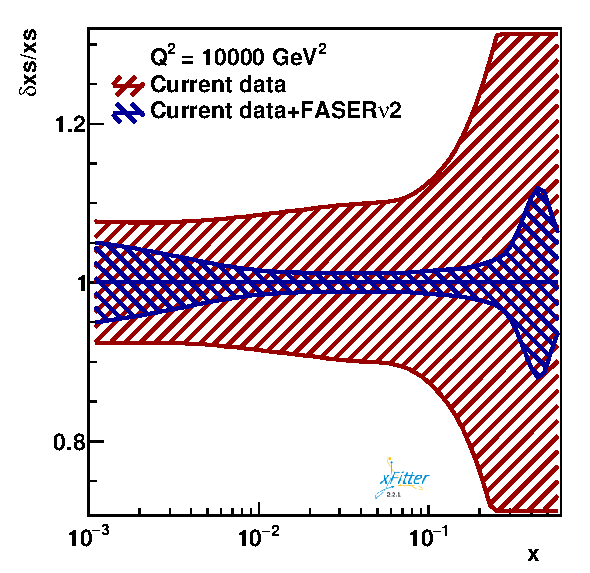
\includegraphics[width=0.32\textwidth]{plots/proton_fasernu2/inclusive+charm_chargediscrimination/statOnly_FASERv2_q2_10000_pdf_s_ratio.pdf}
\caption{The fractional uncertainties (at the 68\% confidence level)
for the up and down valence quarks, total quark singlet, strangeness, charm, and gluon PDFs
in PDF4LHC21 compared to the results of its profiling with the baseline LHC neutrino dataset, namely
FASER$\nu$2 with only statistical errors, both inclusive and charm structure functions, and charge flavour
separation.
%
Results are shown at the scale $Q^2 = 10^4 \, \textrm{GeV}^2$ and the shift in central values
is not considered.}
\label{fig:profiling_baseline}
\end{figure}
%%%%%%%%%%%%%%%%%%%%%%%%%%%%%%%%%%%%%%%%%%%%%%%%%%%%%%%%%%%%%%%%%%%%%%%%

In the following we consider the stability of the results in Fig.~\ref{fig:profiling_baseline}
with respect to the chosen experiment and integrated luminosity, the modelling of systematic
uncertainties, being able to identify or not charm production, and being able to tell part outgoing
charged leptons from anti-leptons.

\paragraph{Dependence with the experiments.}
%
Same as Fig.~\ref{fig:profiling_baseline} comparing FASER$\nu$2 with AdvSND and with FASER$\nu$.

\paragraph{Impact of systematic uncertainties.}
%
The effect of including correlated systematic uncertainties is shown in 
Fig.~\ref{fig:profiling_syst}.
%%%%%%%%%%%%%%%%%%%%%%%%%%%%%%%%%%%%%%%%%%%%%%%%%%%%%%%%%%%%%%%%%%%%%%%%
\begin{figure}[t]
\centering
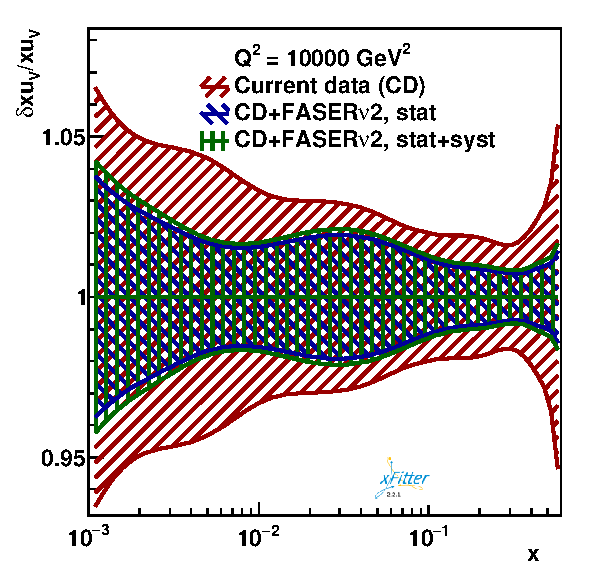
\includegraphics[width=0.32\textwidth]{plots/proton_fasernu2/inclusive+charm_chargediscrimination/syst_FASERv2_q2_10000_pdf_uv_ratio.pdf}
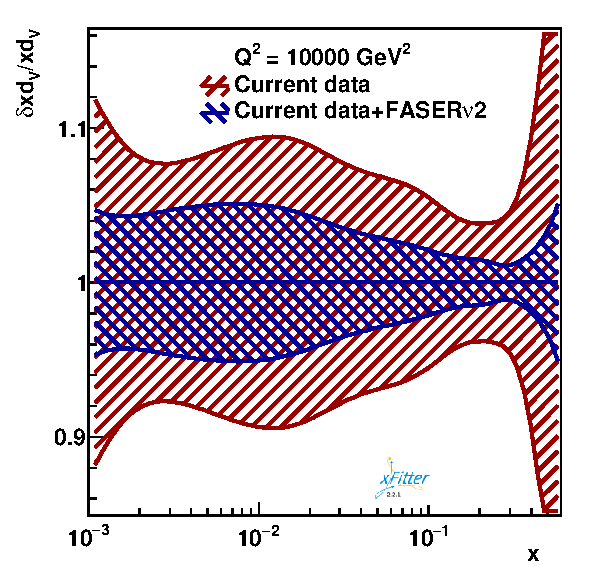
\includegraphics[width=0.32\textwidth]{plots/proton_fasernu2/inclusive+charm_chargediscrimination/syst_FASERv2_q2_10000_pdf_dv_ratio.pdf}
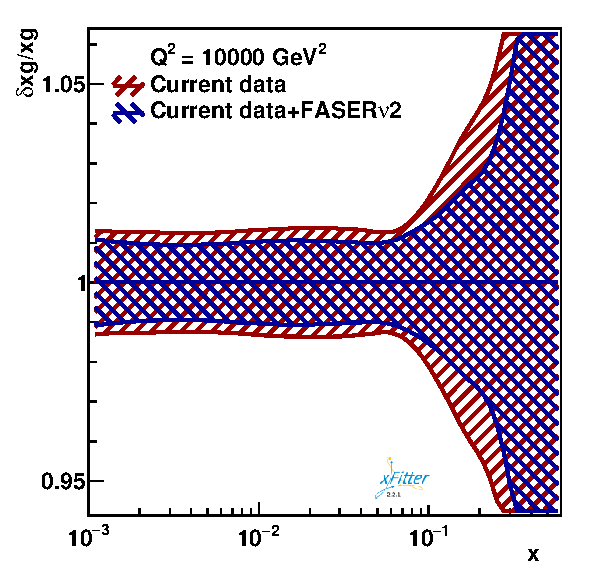
\includegraphics[width=0.32\textwidth]{plots/proton_fasernu2/inclusive+charm_chargediscrimination/syst_FASERv2_q2_10000_pdf_g_ratio.pdf}\\
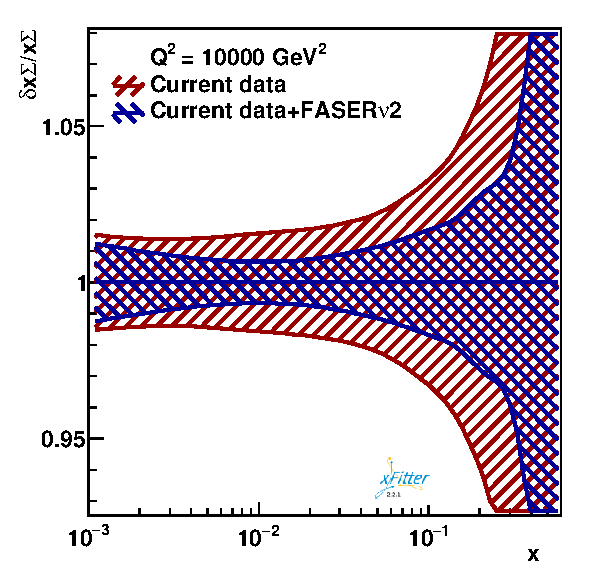
\includegraphics[width=0.32\textwidth]{plots/proton_fasernu2/inclusive+charm_chargediscrimination/syst_FASERv2_q2_10000_pdf_Sea_ratio.pdf}
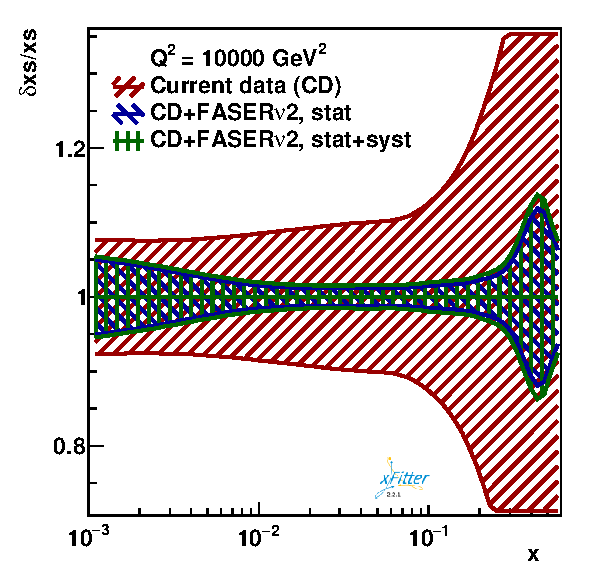
\includegraphics[width=0.32\textwidth]{plots/proton_fasernu2/inclusive+charm_chargediscrimination/syst_FASERv2_q2_10000_pdf_s_ratio.pdf}
\caption{Same as Fig.~\ref{fig:profiling_baseline}, 
but accounting for the statistical as well as correlated systematic uncertainties.
}
\label{fig:profiling_syst}
\end{figure}
%%%%%%%%%%%%%%%%%%%%%%%%%%%%%%%%%%%%%%%%%%%%%%%%%%%%%%%%%%%%%%%%%%%%%%%%

\paragraph{Impact of charm production.}
%
Fig.~\ref{fig:profiling_charm} displays a comparison of the baseline LHC neutrino dataset with the results
of profiling without the charm production structure functions. 
Particularly, the constraints on the $s$ PDF are observed to become more stringent 
by virtue of the contribution of the charm production structure functions.
%%%%%%%%%%%%%%%%%%%%%%%%%%%%%%%%%%%%%%%%%%%%%%%%%%%%%%%%%%%%%%%%%%%%%%%%
\begin{figure}[t]
\centering
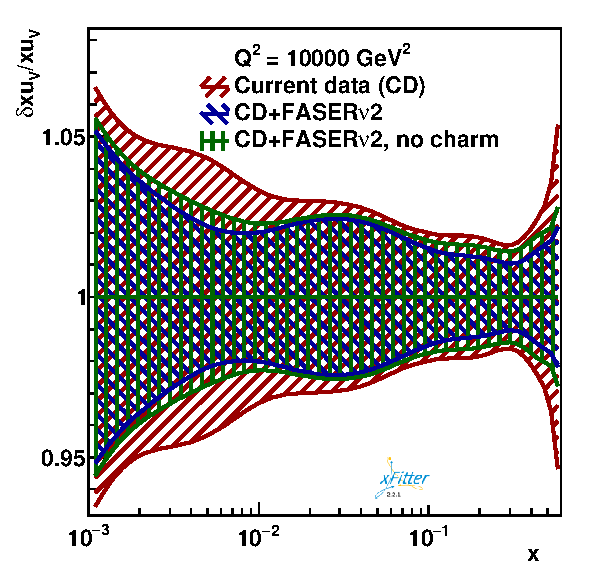
\includegraphics[width=0.32\textwidth]{plots/proton_fasernu2/inclusive-only_vs_inclusive+charm/statOnly_FASERv2_q2_10000_pdf_uv_ratio.pdf}
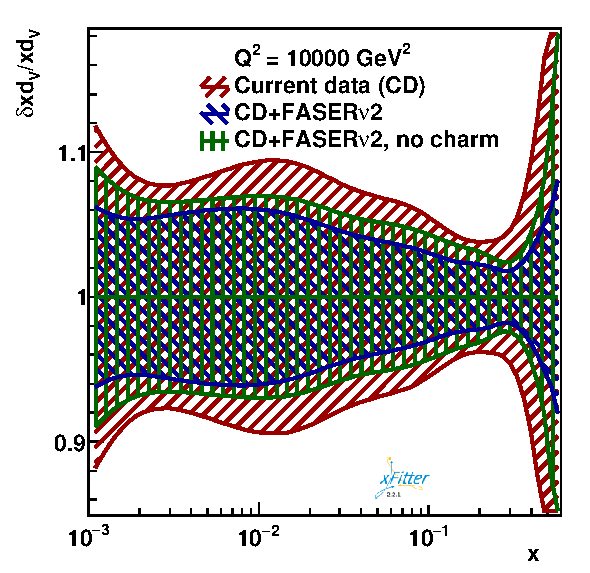
\includegraphics[width=0.32\textwidth]{plots/proton_fasernu2/inclusive-only_vs_inclusive+charm/statOnly_FASERv2_q2_10000_pdf_dv_ratio.pdf}
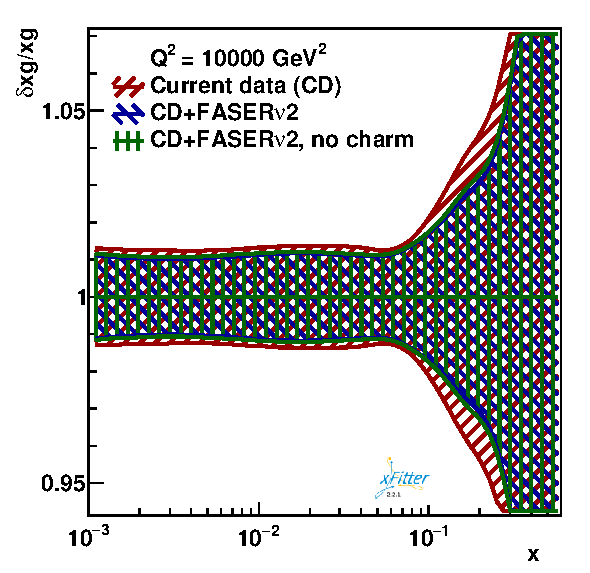
\includegraphics[width=0.32\textwidth]{plots/proton_fasernu2/inclusive-only_vs_inclusive+charm/statOnly_FASERv2_q2_10000_pdf_g_ratio.pdf}\\
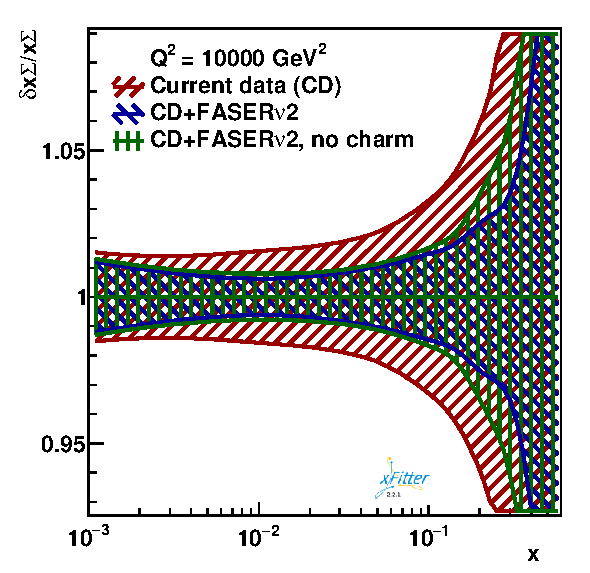
\includegraphics[width=0.32\textwidth]{plots/proton_fasernu2/inclusive-only_vs_inclusive+charm/statOnly_FASERv2_q2_10000_pdf_Sea_ratio.pdf}
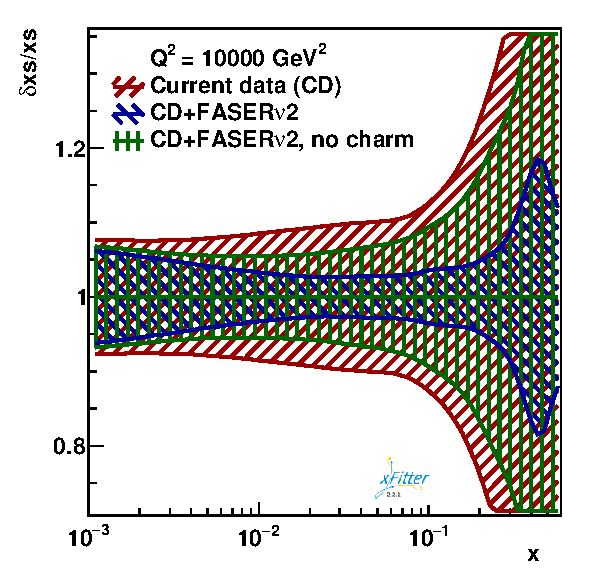
\includegraphics[width=0.32\textwidth]{plots/proton_fasernu2/inclusive-only_vs_inclusive+charm/statOnly_FASERv2_q2_10000_pdf_s_ratio.pdf}
\caption{Comparing the results shown in Fig.~\ref{fig:profiling_baseline} (red and blue), 
to the results obtained without charm production structure functions (green).
}
\label{fig:profiling_charm}
\end{figure}
%%%%%%%%%%%%%%%%%%%%%%%%%%%%%%%%%%%%%%%%%%%%%%%%%%%%%%%%%%%%%%%%%%%%%%%%

\paragraph{The role of lepton charge separation.}
%
Same as Fig.~\ref{fig:profiling_baseline} comparing the baseline LHC neutrino dataset with the results
of a profiling without allowing for the possibility of outgoing lepton charge separation.



\subsection{Impact on NNPDF4.0}
\label{sec:nnpdf40}

Selection of the {\sc\small xFitter} results for the NNPDF case.
